\documentclass[]{beamer}
% Class options include: notes, notesonly, handout, trans,
%                        hidesubsections, shadesubsections,
%                        inrow, blue, red, grey, brown

% Theme for beamer presentation.
\usepackage{beamerthemesplit} 



%%%%%%%%%%%%%%%%%%%%%%%%%%%%%%%%%%%%%%%%%%%%%%%%%%%%%%%%%%%%%%%%%%%%%%



\definecolor{mypink1}{rgb}{0.858, 0.188, 0.478}

\newcommand{\mybox}{%
    \collectbox{%
        \setlength{\fboxsep}{1pt}%
        \fbox{\BOXCONTENT}%
    }%
}

%%%%%%%%%%%%%%%%%%%%%%%%%%%%%%%%%%%%%%%%%%%%%%%%%%%%%%%%%%%%%%%%%%%%%%
% Other themes include: beamerthemebars, beamerthemelined, 
%                       beamerthemetree, beamerthemetreebars  

\title{PHY250: Physics of Shading}    % Enter your title between curly braces
\author{Anabela R. Turlione}                 % Enter your name between curly braces
\institute{Digipen}      % Enter your institute name between curly braces
\date{Fall 2021}                    % Enter the date or \today between curly braces


\begin{document}

% Creates title page of slide show using above information
\begin{frame}
  \titlepage
\end{frame}
%\note{Talk for 30 minutes} % Add notes to yourself that will be displayed when
                           % typeset with the notes or notesonly class options

\section[]{}

% Creates table of contents slide incorporating
% all \section and \subsection commands
% \begin{frame}
%   \tableofcontents
% \end{frame}


% \begin{frame}
%   % \centering
%    \movie[externalviewer]{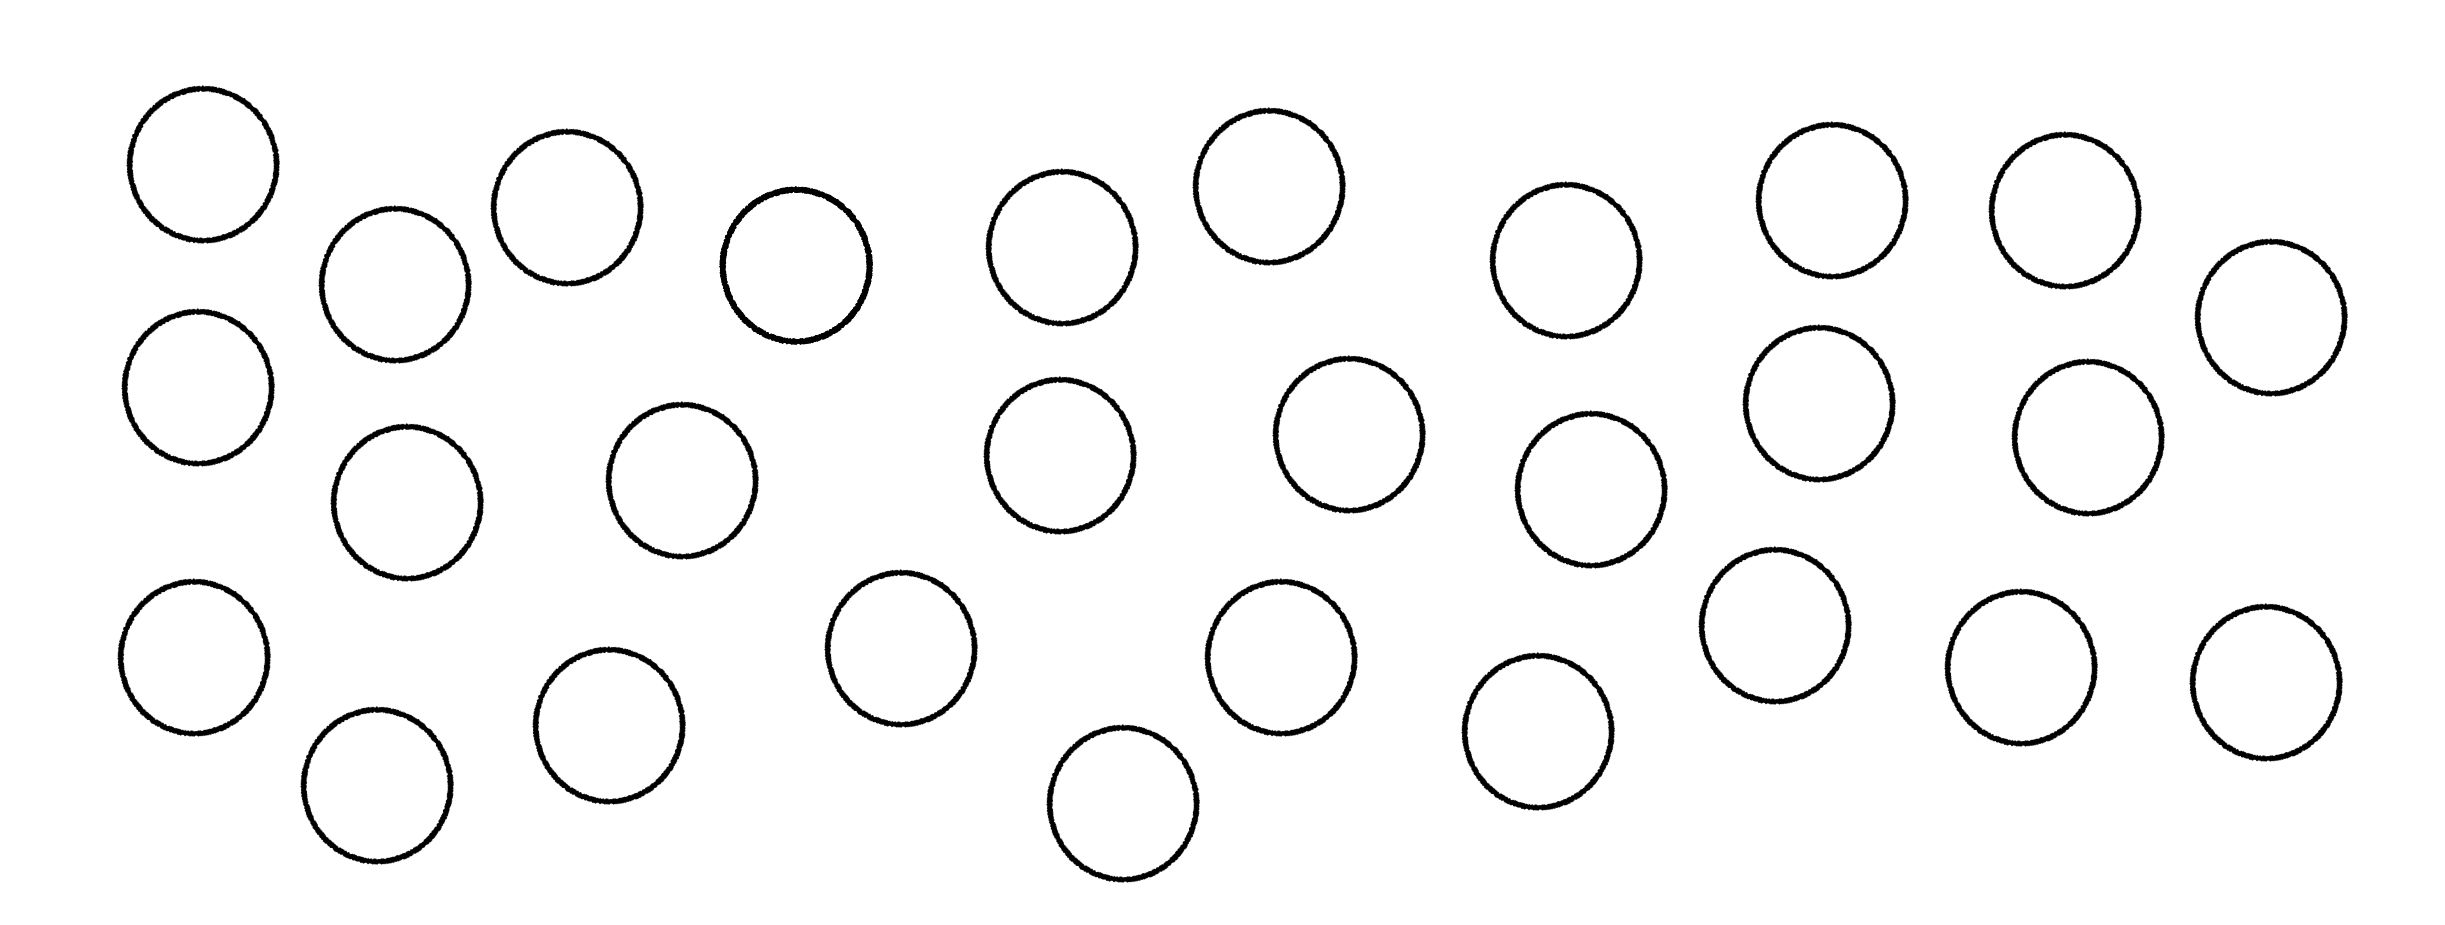
\includegraphics[width=\textheight ,
%    keepaspectratio]{surfacet1.jpg}}{test.mp4}

% \end{frame}
%%%%%%%%%%%%%%%%%%%%%%%%%%%%%%%%%%%%%%%%%%%%%%%%%%%%%%%%%%%%%%%%%%%

%%%%%%%%%%%%%%%%%%%%%%%%%%%%%%%%%%%%%%%%%%%%%%%%%%%%%%%%%%%%%%%%%%%
\newcounter{example}
 \setcounter{example}{1} 


 %%%%%%%%%%%%%%%%%%%%%%%%%%%%%%%%%%%%%%%%%%%%%%%%%%%%%%%%%%%%%%%



 \begin{frame}


  \textcolor{mypink1}{Review: What is light?}
  \begin{figure}[h!]
    \begin{center}
      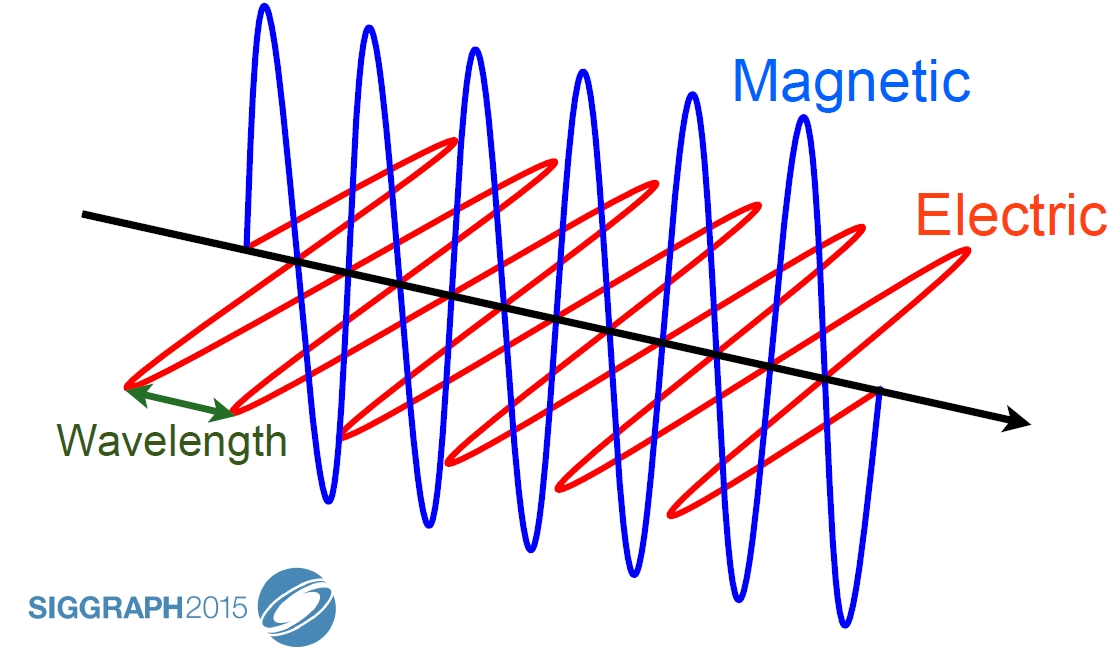
\includegraphics[height=2.5in]{images/1.jpg}
    \end{center}
  \end{figure}
\end{frame}
  
 %%%%%%%%%%%%%%%%%%%%%%%%%%%%%%%%%%%%%%%%%%%%%%%%%%%%%%%%%%%%%%%


 \begin{frame}


    \textcolor{mypink1}{In general, combination of different frequencies}
    \pause

    Example: white light

    \begin{figure}[h!]
      \begin{center}
        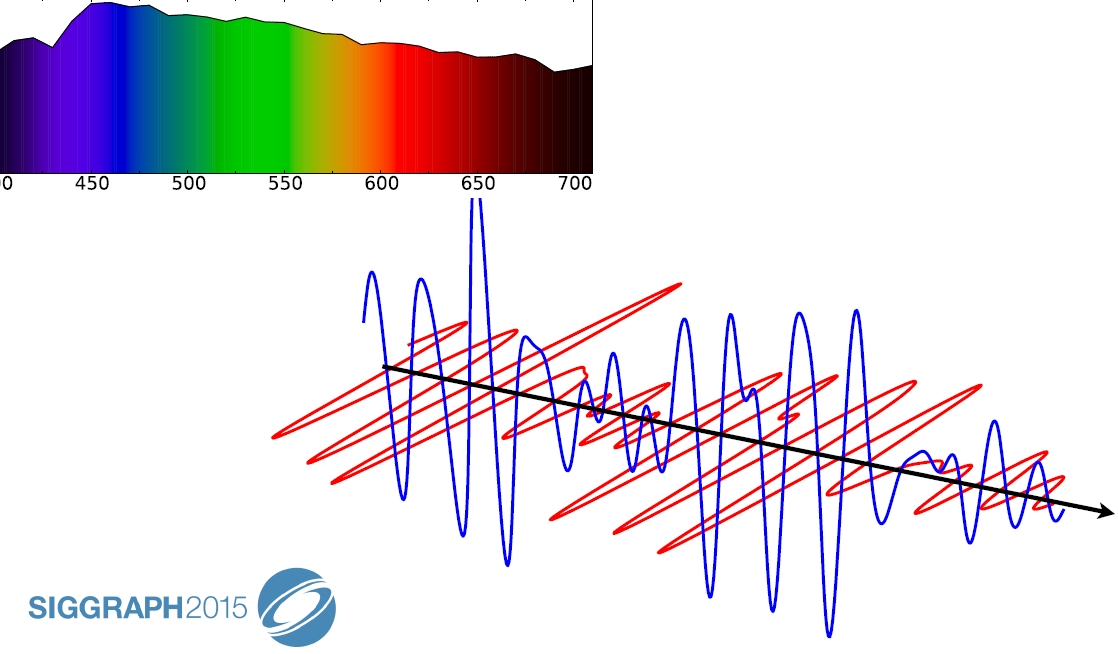
\includegraphics[height=2.5in]{images/2.jpg}
      \end{center}
    \end{figure}
  \end{frame}
    
%%%%%%%%%%%%%%%%%%%%%%%%%%%%%%%%%%%%%%%%%%%%%%%%%%%%%%%%%%%%%%%
 \begin{frame}


    \textcolor{mypink1}{Human vision reduce the infinite-dimension spectrum to a 3D space:}
    \pause

\vspace{5mm}
    Example: white light
    
    \begin{figure}[h!]
      \begin{center}
        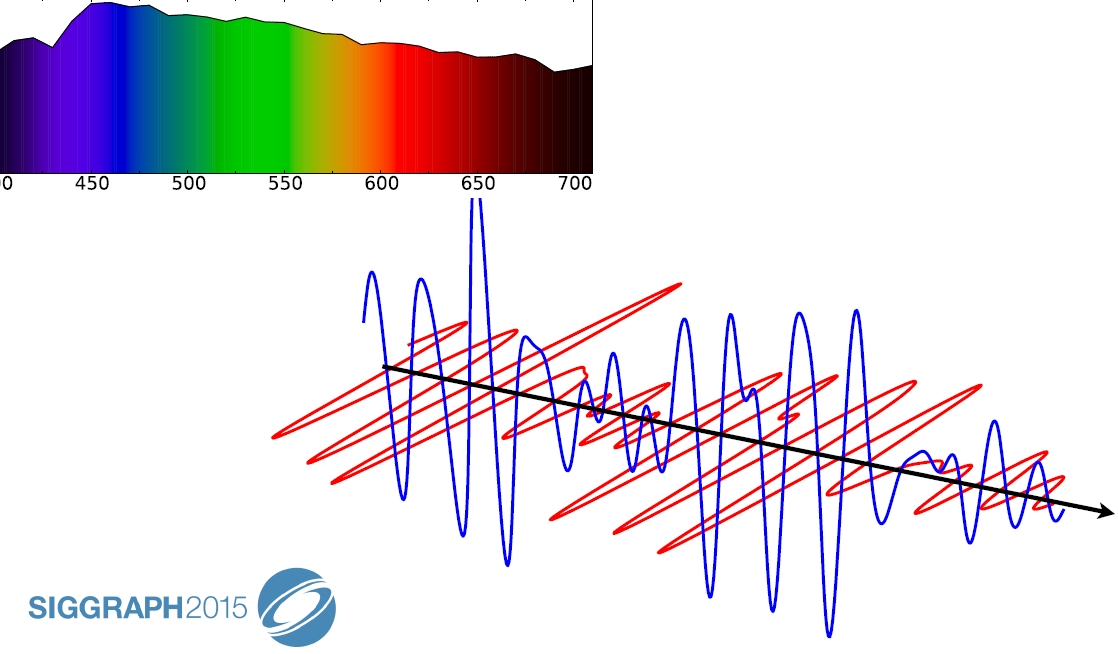
\includegraphics[height=2.5in]{images/2.jpg}
      \end{center}
    \end{figure}
  \end{frame}
    
%%%%%%%%%%%%%%%%%%%%%%%%%%%%%%%%%%%%%%%%%%%%%%%%%%%%%%%%%%%%%%%
   \begin{frame}


    \textcolor{mypink1}{Human vision reduce the infinite-dimension spectrum to a 3D space:}
    \pause

    \vspace{5mm}
    Example: both spectrums give white light
    
    \begin{figure}[h!]
      \begin{center}
        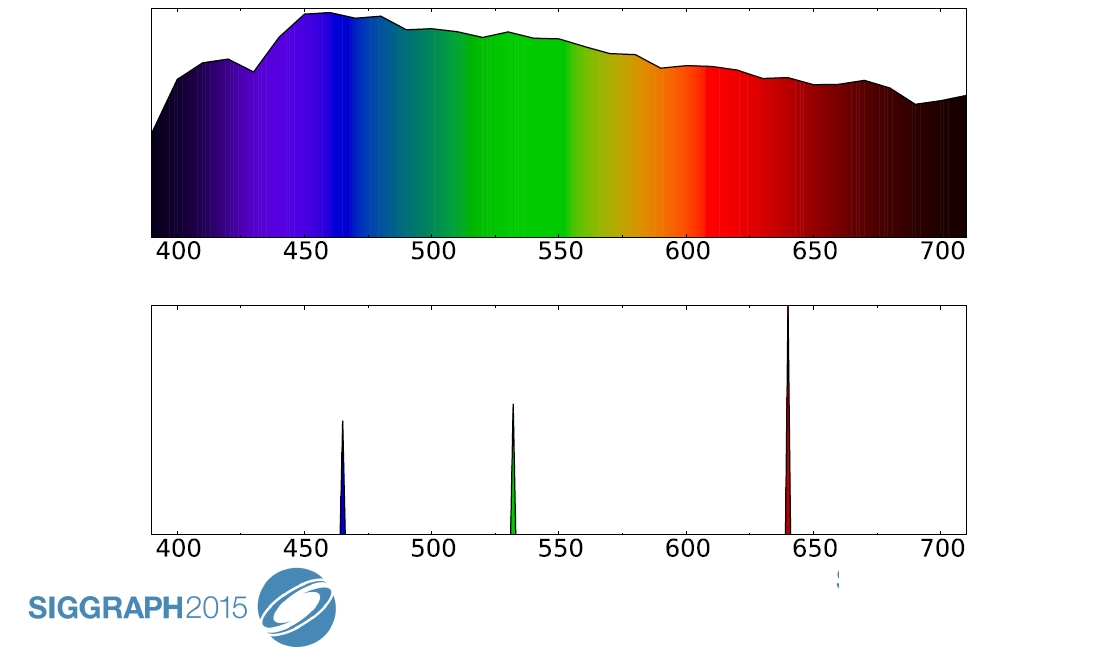
\includegraphics[height=2.5in]{images/3.jpg}
      \end{center}
    \end{figure}
  \end{frame}
    
%%%%%%%%%%%%%%%%%%%%%%%%%%%%%%%%%%%%%%%%%%%%%%%%%%%%%%%%%%%%%%%

   \begin{frame}


    \textcolor{mypink1}{Light interacting with materials:}
    \pause


    
    \begin{figure}[h!]
      \begin{center}
        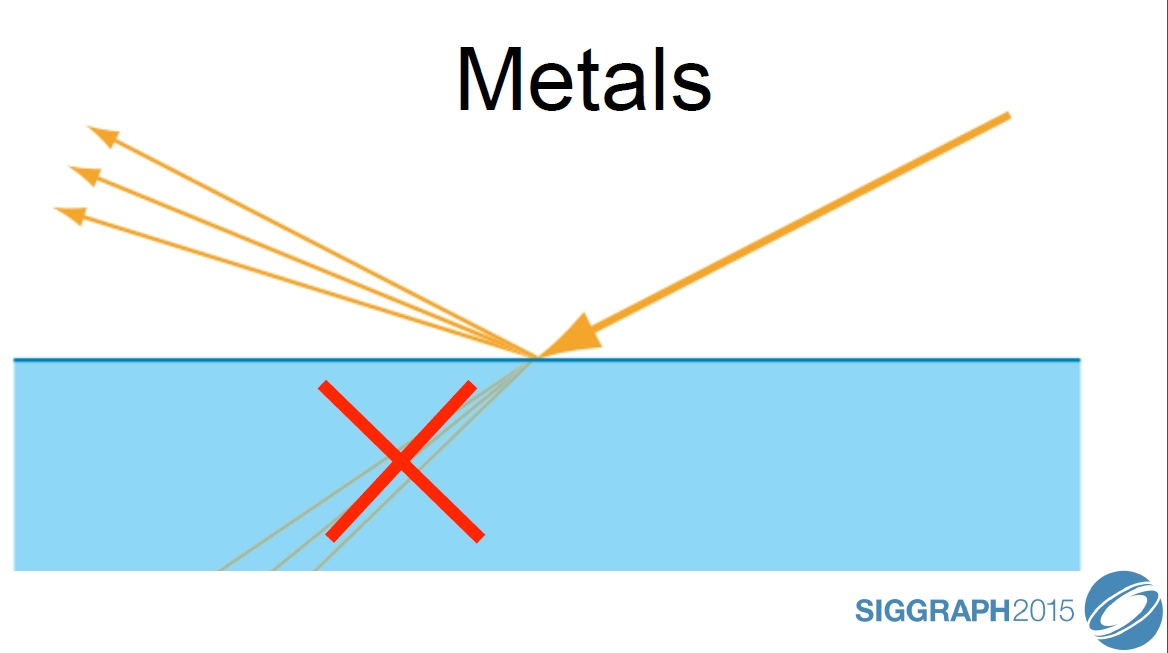
\includegraphics[height=2.5in]{images/4.jpg}
      \end{center}
    \end{figure}
  \end{frame}
    
%%%%%%%%%%%%%%%%%%%%%%%%%%%%%%%%%%%%%%%%%%%%%%%%%%%%%%%%%%%%%%%

\begin{frame}


    \textcolor{mypink1}{Light interacting with materials:}
   

    
    \begin{figure}[h!]
      \begin{center}
        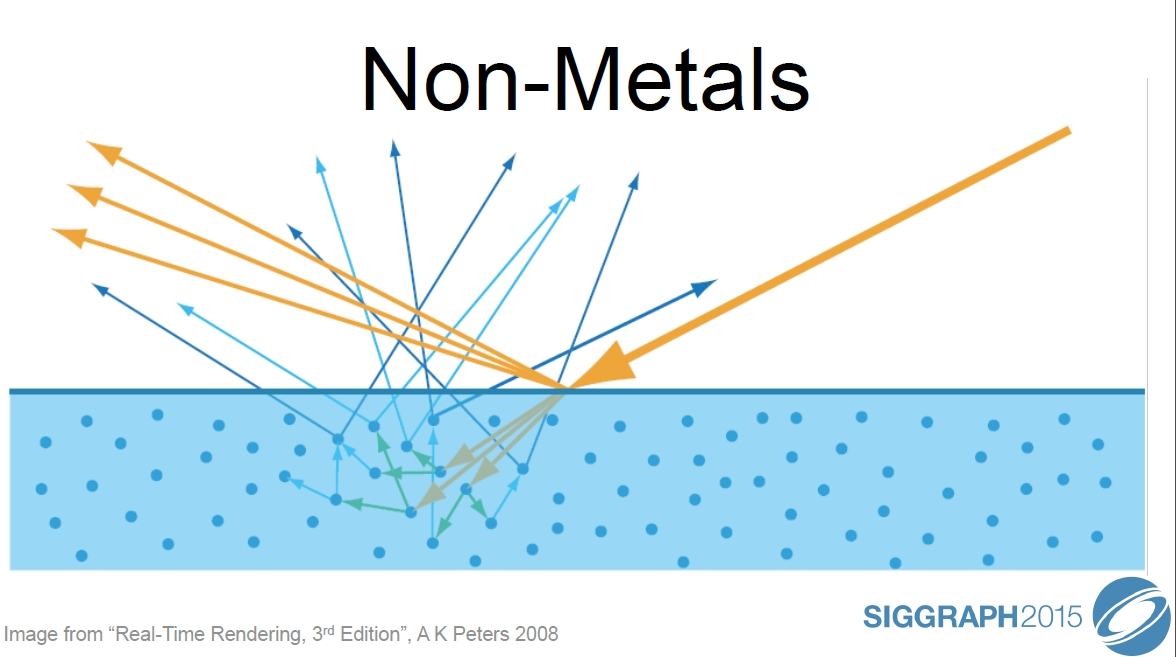
\includegraphics[height=2.5in]{images/5.jpg}
      \end{center}
    \end{figure}
  \end{frame}
    
%%%%%%%%%%%%%%%%%%%%%%%%%%%%%%%%%%%%%%%%%%%%%%%%%%%%%%%%%%%%%%%
\begin{frame}


    \textcolor{mypink1}{Scattering is different from Absoption }
   

    
    \begin{figure}[h!]
      \begin{center}
        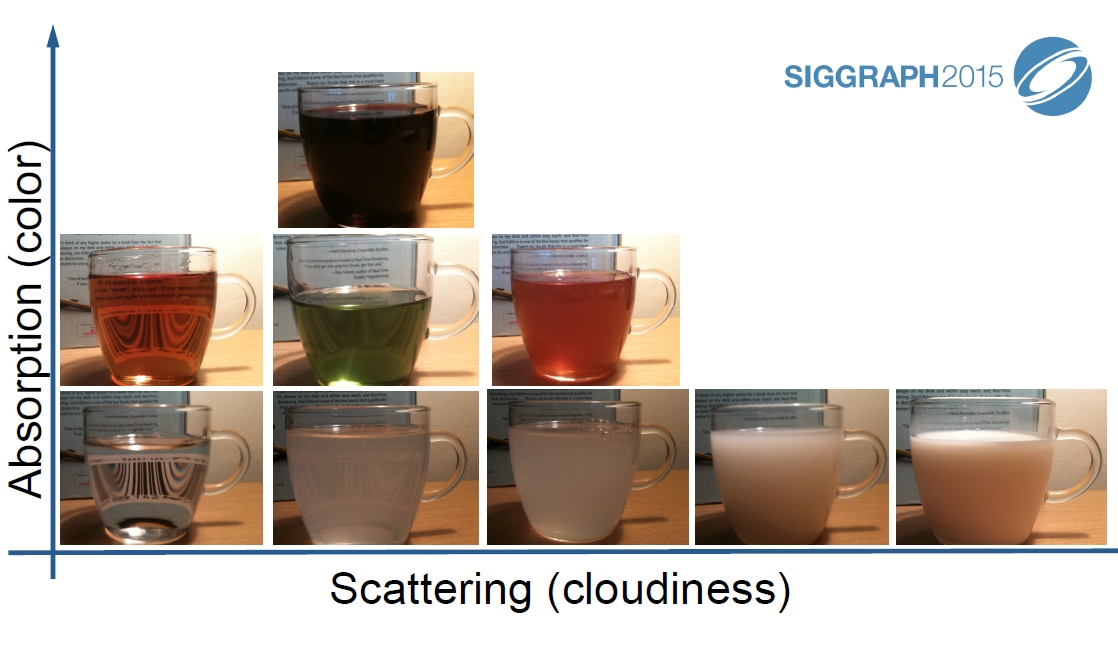
\includegraphics[height=2.5in]{images/6.jpg}
      \end{center}
    \end{figure}
  \end{frame}

  %%%%%%%%%%%%%%%%%%%%%%%%%%%%%%%%%%%%%%%%%%%%%%%%%%%%%%%%%%%%%%%

\begin{frame}


    \textcolor{mypink1}{Perfectly smooth surface }
   

    
    \begin{figure}[h!]
      \begin{center}
        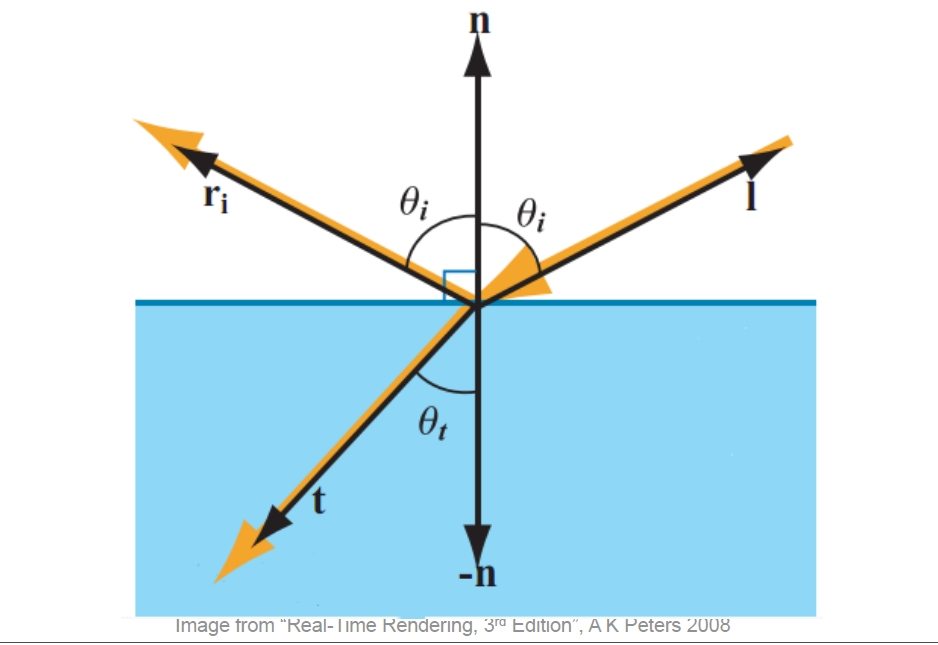
\includegraphics[height=2.2in]{images/11.jpg}
      \end{center}
    \end{figure}
  \end{frame}
    

%%%%%%%%%%%%%%%%%%%%%%%%%%%%%%%%%%%%%%%%%%%%%%%%%%%%%%%%%%%%%%%

\begin{frame}


    \textcolor{mypink1}{Surfaces are not perfectly smooth }
   

    
    \begin{figure}[h!]
      \begin{center}
        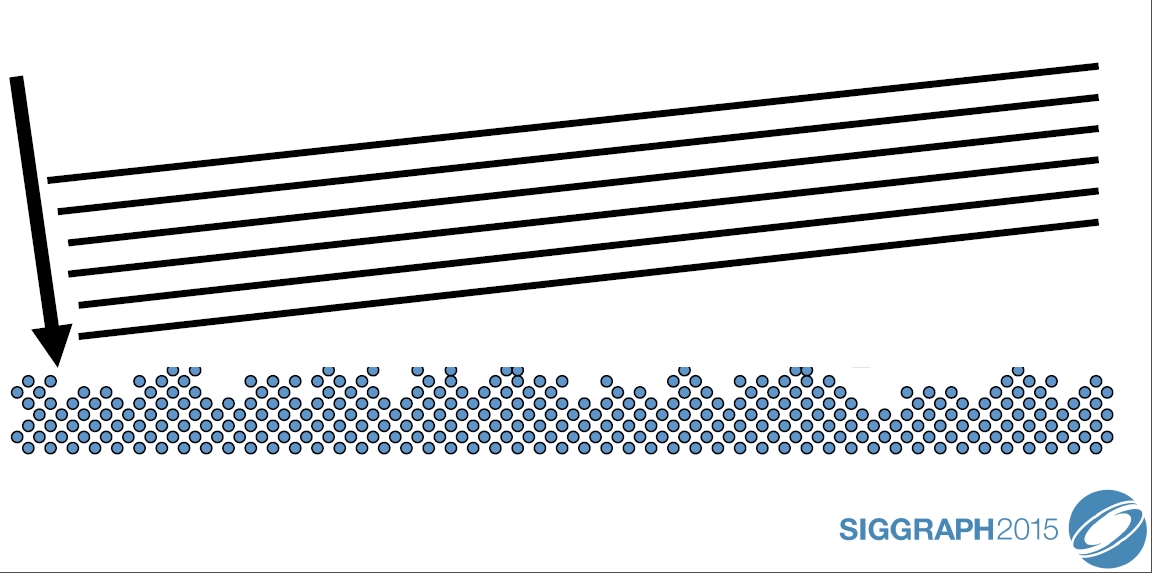
\includegraphics[height=2.2in]{images/7.jpg}
      \end{center}
    \end{figure}
  \end{frame}
    
%%%%%%%%%%%%%%%%%%%%%%%%%%%%%%%%%%%%%%%%%%%%%%%%%%%%%%%%%%%%%%%
\begin{frame}


    \textcolor{mypink1}{Surfaces are not perfectly smooth }
   

    
    \begin{figure}[h!]
      \begin{center}
        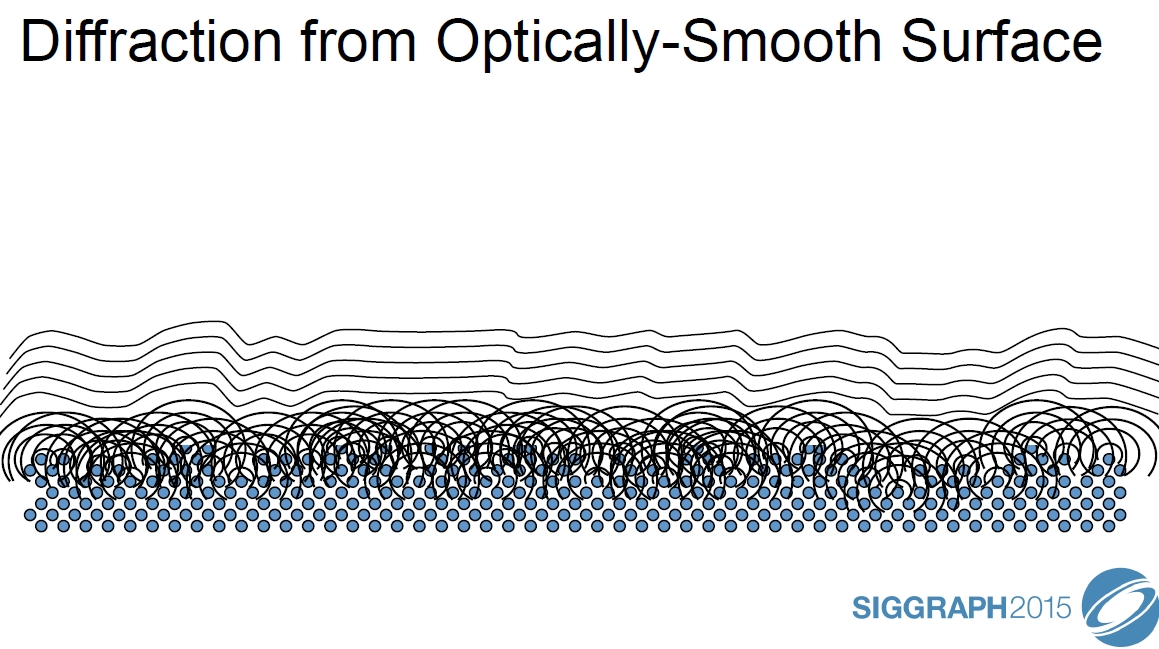
\includegraphics[height=2.5in]{images/8.jpg}
      \end{center}
    \end{figure}
  \end{frame}
    
%%%%%%%%%%%%%%%%%%%%%%%%%%%%%%%%%%%%%%%%%%%%%%%%%%%%%%%%%%%%%%%
\begin{frame}


    \textcolor{mypink1}{Surfaces are not perfectly smooth }
   

    
    \begin{figure}[h!]
      \begin{center}
        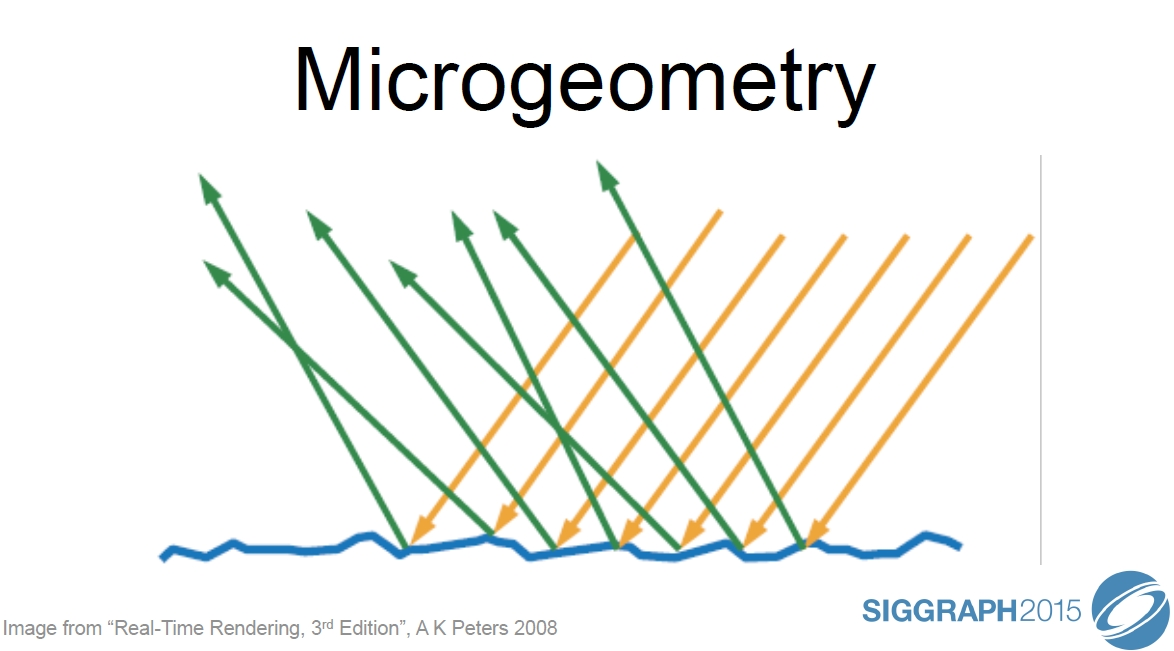
\includegraphics[height=2.2in]{images/9.jpg}
      \end{center}
    \end{figure}
  \end{frame}
    
%%%%%%%%%%%%%%%%%%%%%%%%%%%%%%%%%%%%%%%%%%%%%%%%%%%%%%%%%%%%%%%


\begin{frame}


    \textcolor{mypink1}{Surfaces are not perfectly smooth }
   

    
    \begin{figure}[h!]
      \begin{center}
        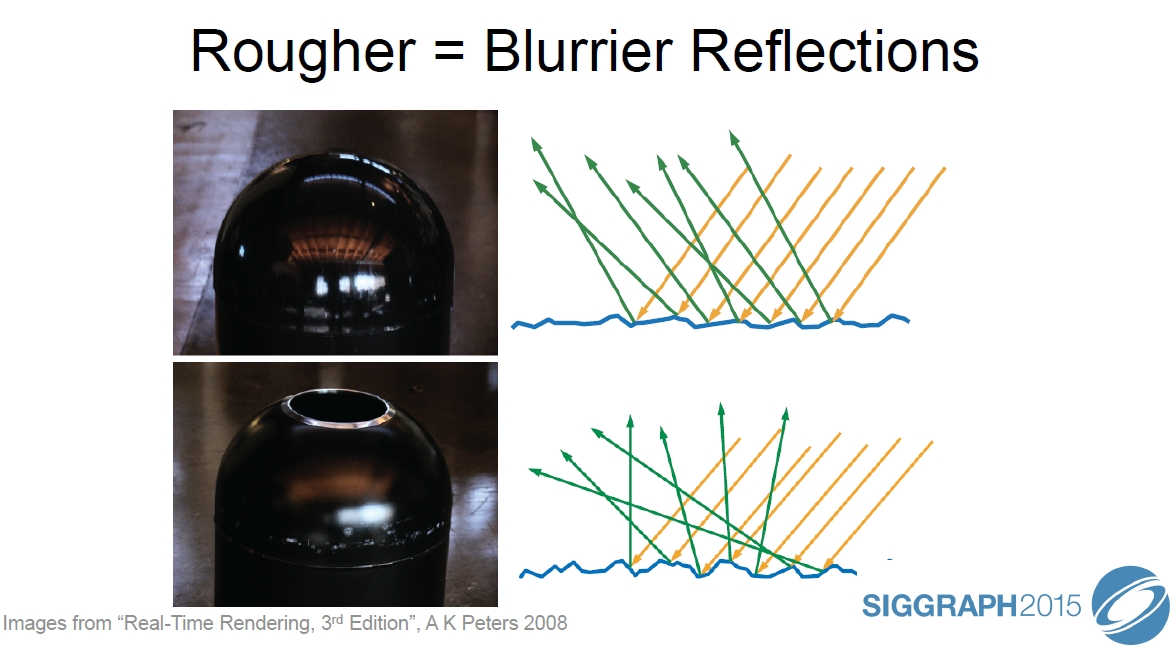
\includegraphics[height=2.5in]{images/10.jpg}
      \end{center}
    \end{figure}
  \end{frame}
    
%%%%%%%%%%%%%%%%%%%%%%%%%%%%%%%%%%%%%%%%%%%%%%%%%%%%%%%%%%%%%%%

\begin{frame}


    \textcolor{mypink1}{Physically Based Rendering (PBR)}
   \pause

   \begin{itemize}
       \item collection of render techniques  based on the same underlying theory.\pause
       \item aims to mimic light in a physically plausible way.\pause
       \item  an approximation of reality\pause
       \item originally explored by Disney and adopted for real-time display by Epic Games \pause
   \end{itemize}


  \end{frame}
    
%%%%%%%%%%%%%%%%%%%%%%%%%%%%%%%%%%%%%%%%%%%%%%%%%%%%%%%%%%%%%%%

\begin{frame}


  \textcolor{mypink1}{The microfacet model}
  \vspace{5mm}
 \pause

 \begin{itemize}
     \item Microfacets \pause $\rightarrow$ little perfectly reflective mirrors. \pause
     \item Rough Surface/Smooth Surface \pause $\rightarrow$ Scattered light or specular reflection.\pause 
 \end{itemize}

\pause
\vspace{5mm}

 \begin{figure}[h!]
  \begin{center}
    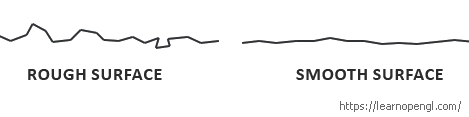
\includegraphics[height=0.9in]{images/13.jpg}
  \end{center}
\end{figure}




\end{frame}
  
%%%%%%%%%%%%%%%%%%%%%%%%%%%%%%%%%%%%%%%%%%%%%%%%%%%%%%%%%%%%%%%

\begin{frame}


  \textcolor{mypink1}{The microfacet model}
\vspace{5mm}

 \begin{itemize}
     \item Microfacets  $\rightarrow$ little perfectly reflective mirrors. 
     \item Rough Surface/Smooth Surface  $\rightarrow$ Scattered light or specular reflection.
 \end{itemize}


\vspace{5mm}

 \begin{figure}[h!]
  \begin{center}
    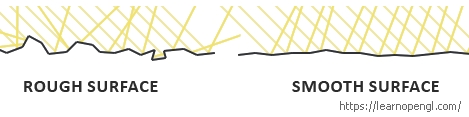
\includegraphics[height=0.9in]{images/12.jpg}
  \end{center}
\end{figure}




\end{frame}

%%%%%%%%%%%%%%%%%%%%%%%%%%%%%%%%%%%%%%%%%%%%%%%%%%%%%%%%%%%%%%%

\begin{frame}


  \textcolor{mypink1}{The microfacet model}
\vspace{5mm}

 \begin{itemize}
     \item On a microscopic level, no surface is completely smooth \pause
     \item We consider that the microfacets are small compared to the pixels.
 \end{itemize}





\end{frame}


%%%%%%%%%%%%%%%%%%%%%%%%%%%%%%%%%%%%%%%%%%%%%%%%%%%%%%%%%%%%%%%

\begin{frame}


  \textcolor{mypink1}{Roughness parameter}
\vspace{5mm}

 

\begin{figure}[h!]
  \begin{center}
    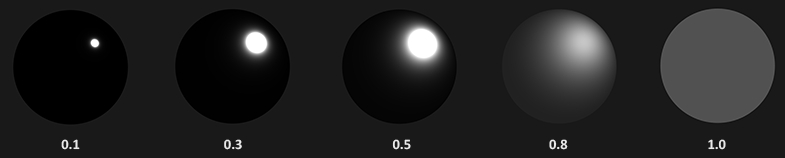
\includegraphics[height=0.9in]{images/14.jpg}
  \end{center}
\end{figure}


\end{frame}

%%%%%%%%%%%%%%%%%%%%%%%%%%%%%%%%%%%%%%%%%%%%%%%%%%%%%%%%%%%%%%%

\begin{frame}


  \textcolor{mypink1}{Energy conservation}
\vspace{5mm}

\begin{itemize}
  \item Outgoing light energy $\leq$ incoming light energy \pause
  \item The bright area increases, but its intensity decreases. \pause
\end{itemize}


\begin{figure}[h!]
  \begin{center}
    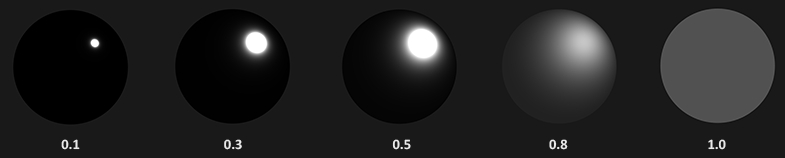
\includegraphics[height=0.9in]{images/14.jpg}
  \end{center}
\end{figure}


\end{frame}

%%%%%%%%%%%%%%%%%%%%%%%%%%%%%%%%%%%%%%%%%%%%%%%%%%%%%%%%%%%%%%%

\begin{frame}


  \textcolor{mypink1}{Difuffe light $\neq$ Specular light} 
\vspace{5mm}

\begin{figure}[h!]
  \begin{center}
    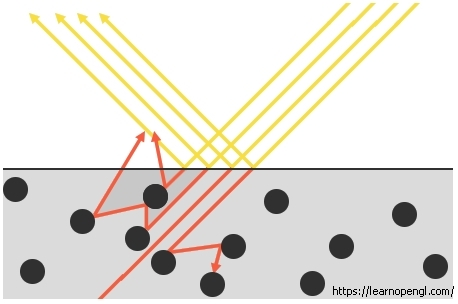
\includegraphics[height=1.9in]{images/15.jpg}
  \end{center}
\end{figure}



\end{frame}

%%%%%%%%%%%%%%%%%%%%%%%%%%%%%%%%%%%%%%%%%%%%%%%%%%%%%%%%%%%%%%%

\begin{frame}


  \textcolor{mypink1}{Difuffe light $\neq$ Specular light} 
\vspace{5mm}

\begin{figure}[h!]
  \begin{center}
    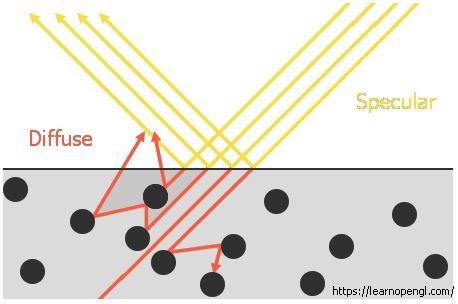
\includegraphics[height=1.9in]{images/16.jpg}
  \end{center}
\end{figure}



\end{frame}

%%%%%%%%%%%%%%%%%%%%%%%%%%%%%%%%%%%%%%%%%%%%%%%%%%%%%%%%%%%%%%%

\begin{frame}


  \textcolor{mypink1}{Difuffe light $\neq$ Specular light} 
\vspace{5mm}

\begin{figure}[h!]
  \begin{center}
    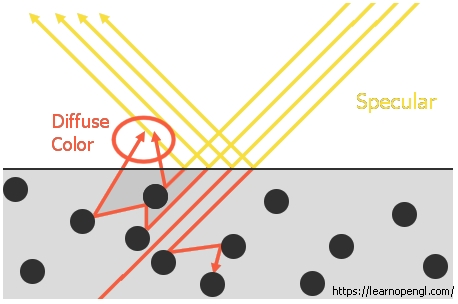
\includegraphics[height=1.9in]{images/17.jpg}
  \end{center}
\end{figure}



\end{frame}

%%%%%%%%%%%%%%%%%%%%%%%%%%%%%%%%%%%%%%%%%%%%%%%%%%%%%%%%%%%%%%%

\begin{frame}


  \textcolor{mypink1}{Difuffe light $\neq$ Specular light} 
\vspace{5mm}
\pause

\begin{itemize}
  \item Physically based rendering \pause $\rightarrow$ all refracted light gets absorbed and scattered at a very small area of impact (nearest neighbor algorithm).\pause
  \item In metals \pause $\rightarrow$ no scattering  \pause $\rightarrow$  they are treated differently in the PBR pipeline.\pause
  \item The energy of the refracted light is the Total energy - reflective light$\pause \rightarrow$ amount of light refracted.
\end{itemize}


\end{frame}

%%%%%%%%%%%%%%%%%%%%%%%%%%%%%%%%%%%%%%%%%%%%%%%%%%%%%%%%%%%%%%%

\begin{frame}


  \textcolor{mypink1}{The reflectance equation} 
\vspace{5mm}
\pause

\begin{itemize}
  \item Rendering Equation \pause The best model to simulate the visuals of light.
  \item PBR follows a more specialized version:\pause the reflectance equation.
\end{itemize}



\end{frame}

%%%%%%%%%%%%%%%%%%%%%%%%%%%%%%%%%%%%%%%%%%%%%%%%%%%%%%%%%%%%%%%

\begin{frame}


  \textcolor{mypink1}{Definitions} 
\vspace{5mm}
\pause


\begin{itemize}
  \item Radiance: magnitude of light coming from one direction.\pause
  \item Radiant Flux: $\Phi$, transmitted energy of a light source measured in Watts.\pause
  \item Solid Angle $\omega$: \pause  area of a shape projected onto a unit sphere
\end{itemize}



\begin{figure}[h!]
  \begin{center}
    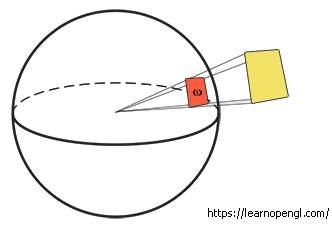
\includegraphics[height=1.5in]{images/18.jpg}
  \end{center}
\end{figure}

\end{frame}


%%%%%%%%%%%%%%%%%%%%%%%%%%%%%%%%%%%%%%%%%%%%%%%%%%%%%%%%%%%%%%%


\begin{frame}


  \textcolor{mypink1}{Definitions} 
\vspace{5mm}
\pause


\begin{itemize}
  \item Radiant intensity: amount of radiant flux per solid angle, 
\end{itemize}

\begin{equation*}
  I=\frac{d\Phi}{d \omega}
\end{equation*}

\begin{figure}[h!]
  \begin{center}
    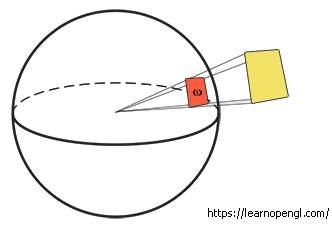
\includegraphics[height=1.5in]{images/18.jpg}
  \end{center}
\end{figure}

\end{frame}


%%%%%%%%%%%%%%%%%%%%%%%%%%%%%%%%%%%%%%%%%%%%%%%%%%%%%%%%%%%%%%%


\begin{frame}


  \textcolor{mypink1}{Radiance} 
\vspace{5mm}
\pause


\begin{itemize}
  \item Radiance is described as the total observed energy in an area A.\pause
  \item Small A $\pause \rightarrow$ Radiance in a point $p$
\end{itemize}

\pause

\begin{equation*}
  L=\frac{d^2\Phi}{d Ad \omega cos \theta}
\end{equation*}

\begin{figure}[h!]
  \begin{center}
    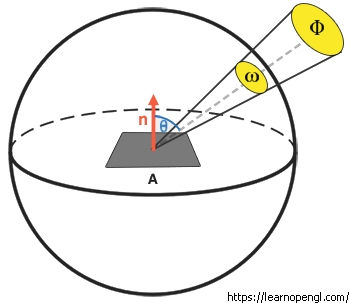
\includegraphics[height=1.7in]{images/19.jpg}
  \end{center}
\end{figure}

\end{frame}


%%%%%%%%%%%%%%%%%%%%%%%%%%%%%%%%%%%%%%%%%%%%%%%%%%%%%%%%%%%%%%%



\begin{frame}
  \textcolor{mypink1}{What is the radiance then?} 
\pause
  \begin{enumerate}
    \item  it is a radiometric measure of the amount of light in an area.\pause
    \item  it  is strongest when it is directly perpendicular to the surface.

  \end{enumerate}







\end{frame}


%%%%%%%%%%%%%%%%%%%%%%%%%%%%%%%%%%%%%%%%%%%%%%%%%%%%%%%%%%%%%%%



\begin{frame}


  The reflectance equation then is the sum of all incoming radiance  within an hemisphere $\omega$

\vspace{5mm}
\pause

  \begin{figure}[h!]
    \begin{center}
      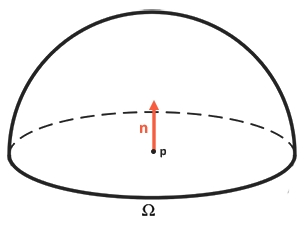
\includegraphics[height=1.7in]{images/20.jpg}
    \end{center}
  \end{figure}
  
  
  \end{frame}

%%%%%%%%%%%%%%%%%%%%%%%%%%%%%%%%%%%%%%%%%%%%%%%%%%%%%%%%%%%%%%%



\begin{frame}
  \textcolor{mypink1}{Reflectance Equation} 
\pause
\vspace{5mm}
                                                

\begin{equation*}
  L_0=\int_{\Omega}f_r(p,\omega_i,\omega_0)L_i(p,\omega_i)n\cdot\omega_id\omega_i
\end{equation*}

\vspace{5mm}

\pause
$f:$ bidirectional reflective distribution function (BRDF), depends on the material .
\pause
\vspace{5mm}

$L_0$  measures the reflected sum of the lights' irradiance onto point p as viewed from $\omega_0$.

\end{frame}
%%%%%%%%%%%%%%%%%%%%%%%%%%%%%%%%%%%%%%%%%%%%%%%%%%%%%%%%%%%%%%%



\begin{frame}
  \textcolor{mypink1}{Function $f$: bidirectional reflective distribution} 
  \vspace{7mm}

  \pause
  The BRDF approximates how much each individual light ray 
  $\omega_i$ contributes to the final reflected light of an opaque surface given its material properties. 
  \vspace{5mm}


  \pause
\vspace{5mm}

  Perfectly smooth surface \pause $\rightarrow  BRDF = 0.0$ for  all incoming light rays   except the one ray that has the same (reflected) angle as the outgoing ray   $\omega_0,~\rightarrow BRDF=1.0$ .


  
  
\end{frame}


%%%%%%%%%%%%%%%%%%%%%%%%%%%%%%%%%%%%%%%%%%%%%%%%%%%%%%%%%%%%%%%



\begin{frame}
  \textcolor{mypink1}{Function $f$: bidirectional reflective distribution} 
  \vspace{7mm}



\begin{itemize}
  \item Function: $f_r(p,\omega_i,\omega_0)$.\pause
  \item input: incoming light, direction $\omega_i$ \pause
  \item outgoing direction: $\omega_0$ \pause
\end{itemize}

  
  
\end{frame}
%%%%%%%%%%%%%%%%%%%%%%%%%%%%%%%%%%%%%%%%%%%%%%%%%%%%%%%%%%%%%%%



\begin{frame}
  \textcolor{mypink1}{Function $f$: bidirectional reflective distribution} 
  \vspace{7mm}

This function depends on:\pause
\begin{itemize}
  \item Normal distribution function: approximates the amount the surface's microfacets are aligned.\pause
  \item Geometry function: Describes the self-shadowing property of the microfacets. \pause
  \item Fresnel equation: The Fresnel equation describes the ratio of surface reflection at different surface angles.\pause
\end{itemize}
  
  
\end{frame}

%%%%%%%%%%%%%%%%%%%%%%%%%%%%%%%%%%%%%%%%%%%%%%%%%%%%%%%%%%%%%%%



\begin{frame}
  \textcolor{mypink1}{Normal Distribution} 
  \vspace{7mm}

  \begin{figure}[h!]
    \begin{center}
      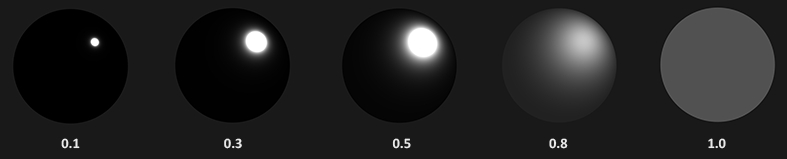
\includegraphics[height=0.9in]{images/21.jpg}
    \end{center}
  \end{figure}
  
\end{frame}

%%%%%%%%%%%%%%%%%%%%%%%%%%%%%%%%%%%%%%%%%%%%%%%%%%%%%%%%%%%%%%%



\begin{frame}
  \textcolor{mypink1}{Geometry Function} 
  \vspace{7mm}

  \begin{figure}[h!]
    \begin{center}
      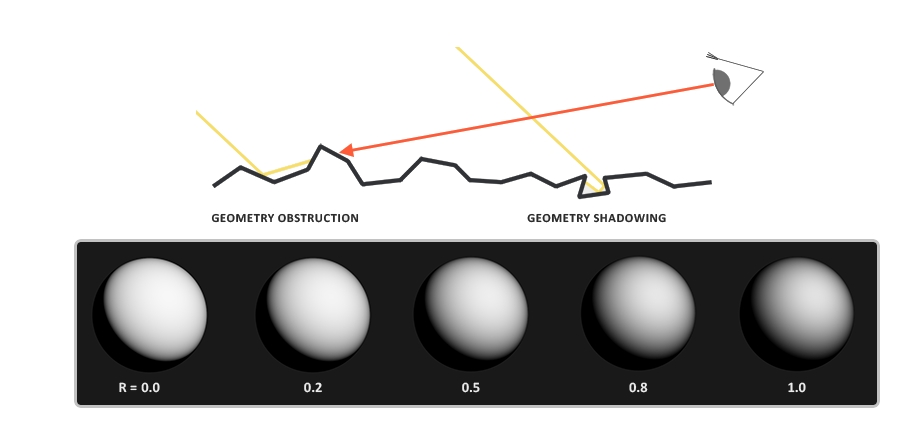
\includegraphics[height=2.in]{images/22.jpg}
    \end{center}
  \end{figure}
  
\end{frame}
%%%%%%%%%%%%%%%%%%%%%%%%%%%%%%%%%%%%%%%%%%%%%%%%%%%%%%%%%%%%%%%



\begin{frame}
  \textcolor{mypink1}{Fresnel Equation} 
  \vspace{7mm}

  \begin{enumerate}
    \item Look at your desk from a perpendicular view angle.\pause
    \item Then look at it from an angle.\pause
    \item An almost 90 degree angle you'll see the reflections become much more apparent. \pause
    \item All surfaces theoretically fully reflect light if seen from perfect 90-degree angles.\pause
  \end{enumerate}
  
  \vspace{7mm}

  
 This phenomenon is known as Fresnel and is described by the \textbf{Fresnel equation}.
\end{frame}


%%%%%%%%%%%%%%%%%%%%%%%%%%%%%%%%%%%%%%%%%%%%%%%%%%%%%%%%%%%%%%%



\begin{frame}
  \textcolor{mypink1}{Fresnel Equation} 
  \vspace{7mm}

\begin{equation*}
  F=F_0+(1-F_0)(1-(h\cdot v))^5
\end{equation*}
\pause
\vspace{10mm}

$F_0:$ Base reflectivity (depends on the IOR)
\pause
\vspace{5mm}

\begin{figure}[h!]
  \begin{center}
    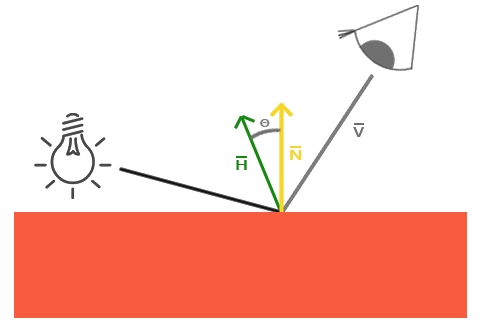
\includegraphics[height=1.7in]{images/23.jpg}
  \end{center}
\end{figure}

\end{frame}

%%%%%%%%%%%%%%%%%%%%%%%%%%%%%%%%%%%%%%%%%%%%%%%%%%%%%%%%%%%%%%%
 \end{document}
%%%%%%%%%%%%%%%%%%%%%%%%%%%%%%%%%%%%%%%%%%%%%%%%%%%%%%%%%%%%%%%